%% ----------------------------------------------------------------
%% Article.tex
%% ---------------------------------------------------------------- 
\documentclass{ecsarticle}     % Use the Article Style
\graphicspath{{../Figures/}}   % Location of your graphics files
\usepackage{natbib}            % Use Natbib style for the refs.
\hypersetup{colorlinks=true}   % Set to false for black/white printing
\input{Definitions}            % Include your abbreviations
%% ----------------------------------------------------------------
\begin{document}
\frontmatter
\title      {An Investigation into \dots}
\authors    {\texorpdfstring
             {\href{mailto:S.R.Gunn@ecs.soton.ac.uk}{Steve R. Gunn}}
             {Steve R. Gunn}
            }
\addresses  {\groupname\\\deptname\\\univname}
\date       {\today}
\subject    {}
\keywords   {}
\maketitle
\begin{abstract}
This work is all about \dots
\end{abstract}
\tableofcontents
\listoffigures
\listoftables
\lstlistoflistings
\listofsymbols{ll}{$w$ & The weight vector}
\mainmatter
%% ----------------------------------------------------------------
\section{Introduction} \label{Section:Introduction}
You probably found all the files from \cite{Gunn:2001:pdflatex}.
\tref{Table:tabex} illustrates the results of my work.
\begin{table}[!htb]
  \centering
  \begin{tabular}{cc}
  \toprule
  \textbf{Training Error} & \textbf{Testing Error}\\
  \midrule
  0 & $\infty$\\
  \bottomrule
  \end{tabular}
  \caption{The Results}
  \label{Table:tabex}
\end{table}

\fref{Figure:figex} shows why this is the case.
\begin{figure}[!htb]
  \centering
  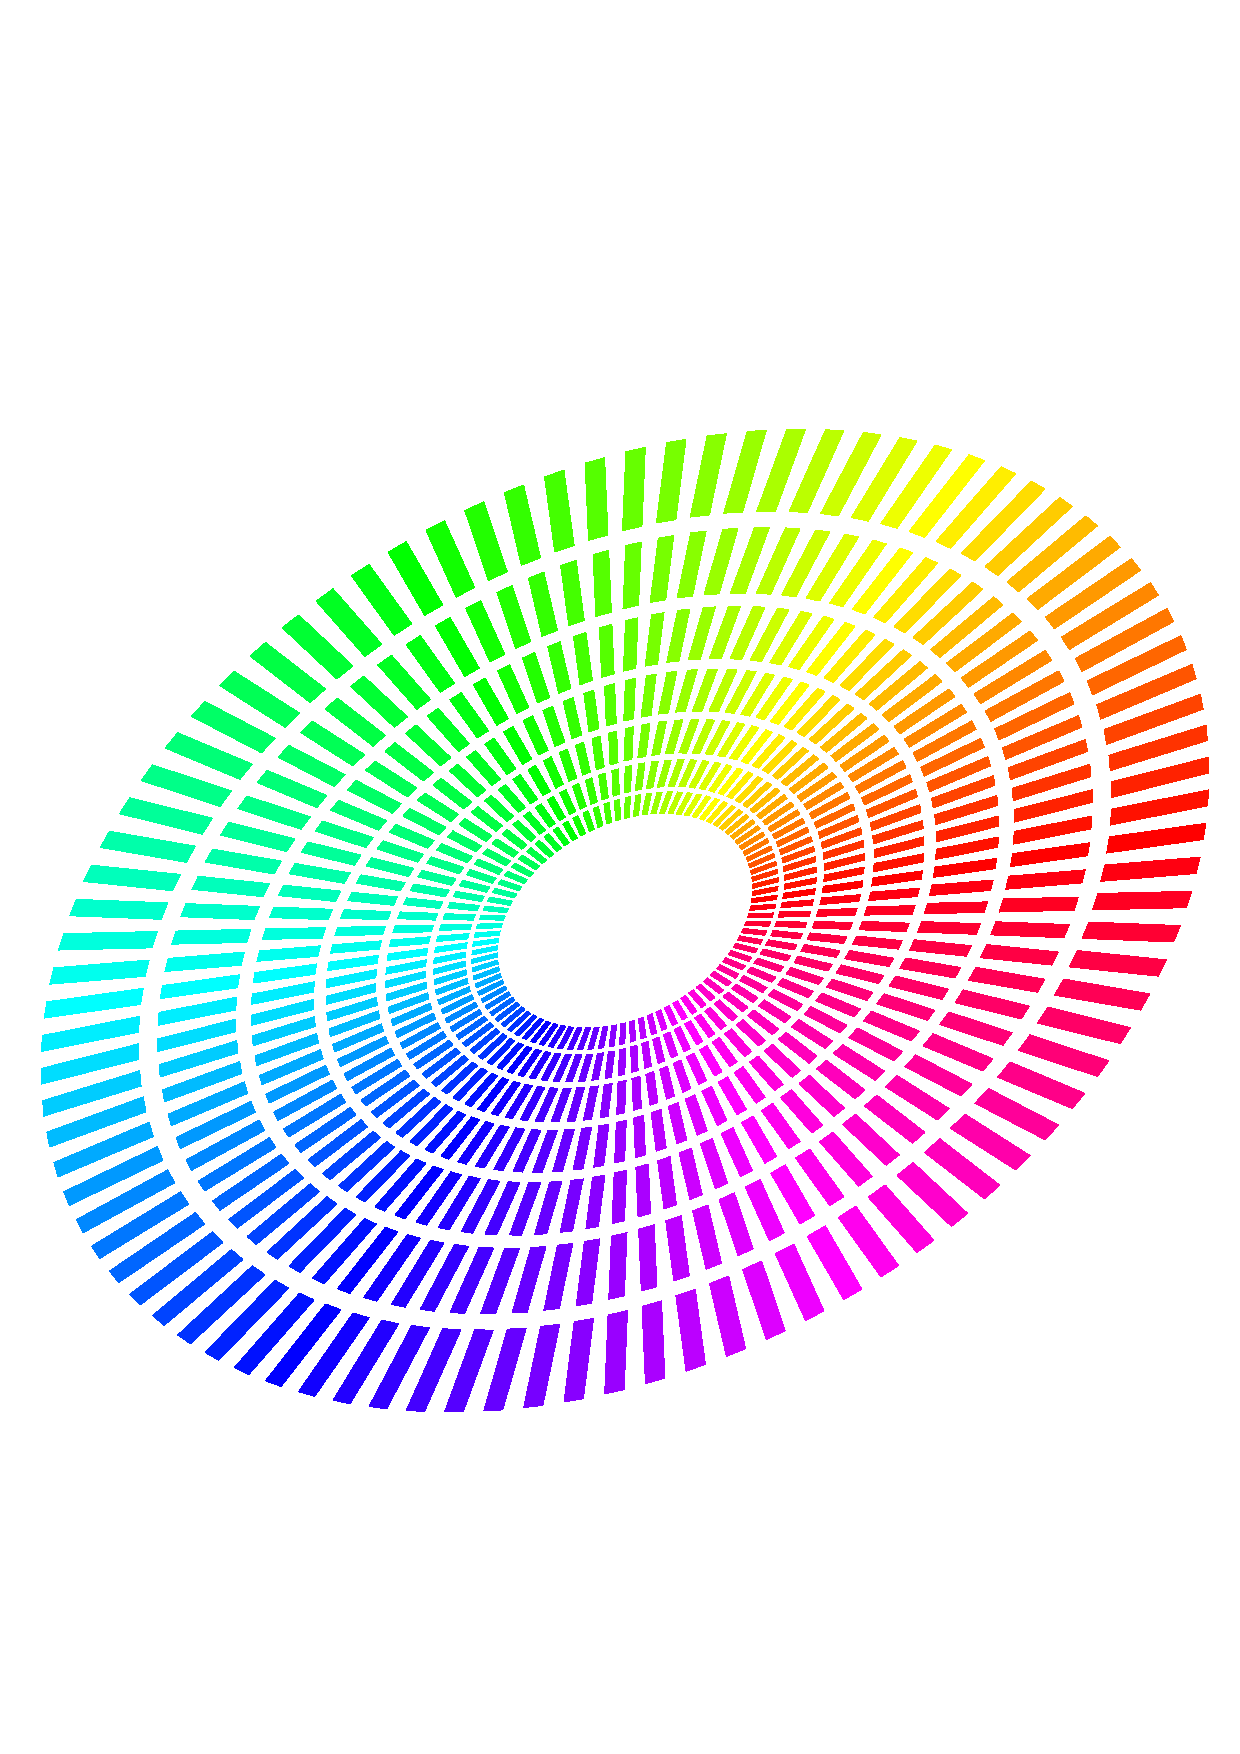
\includegraphics[width=8cm]{figure}
  \caption{A colourful picture.}
  \label{Figure:figex}
\end{figure}

This page shows you a subfigure example in \fref{Figure:figsubex}.
\begin{figure}[!htb]
  \centering
  \subfigure[The left caption]{
    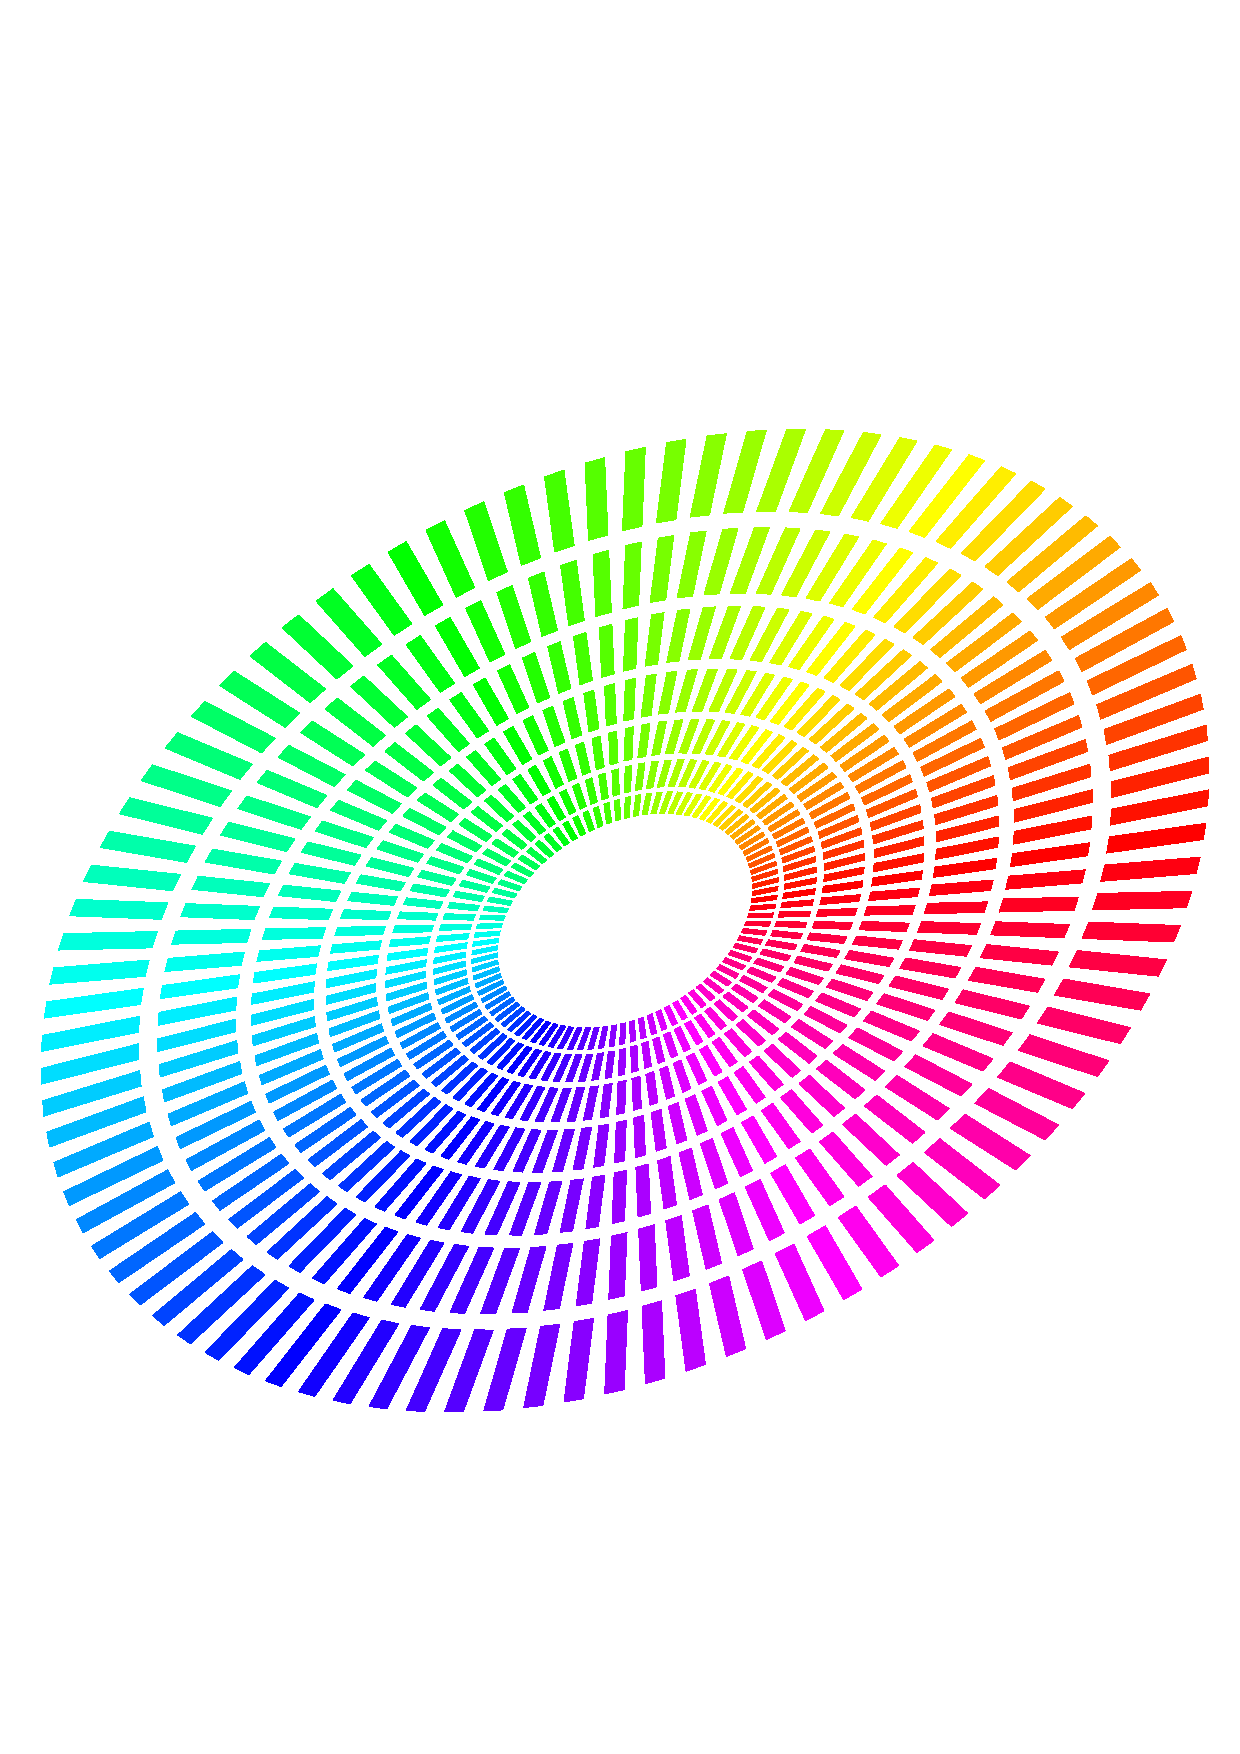
\includegraphics[width=4.2cm]{figure}
    \label{Figure:figsubex:left}
  }
  \subfigure[The right caption]{
    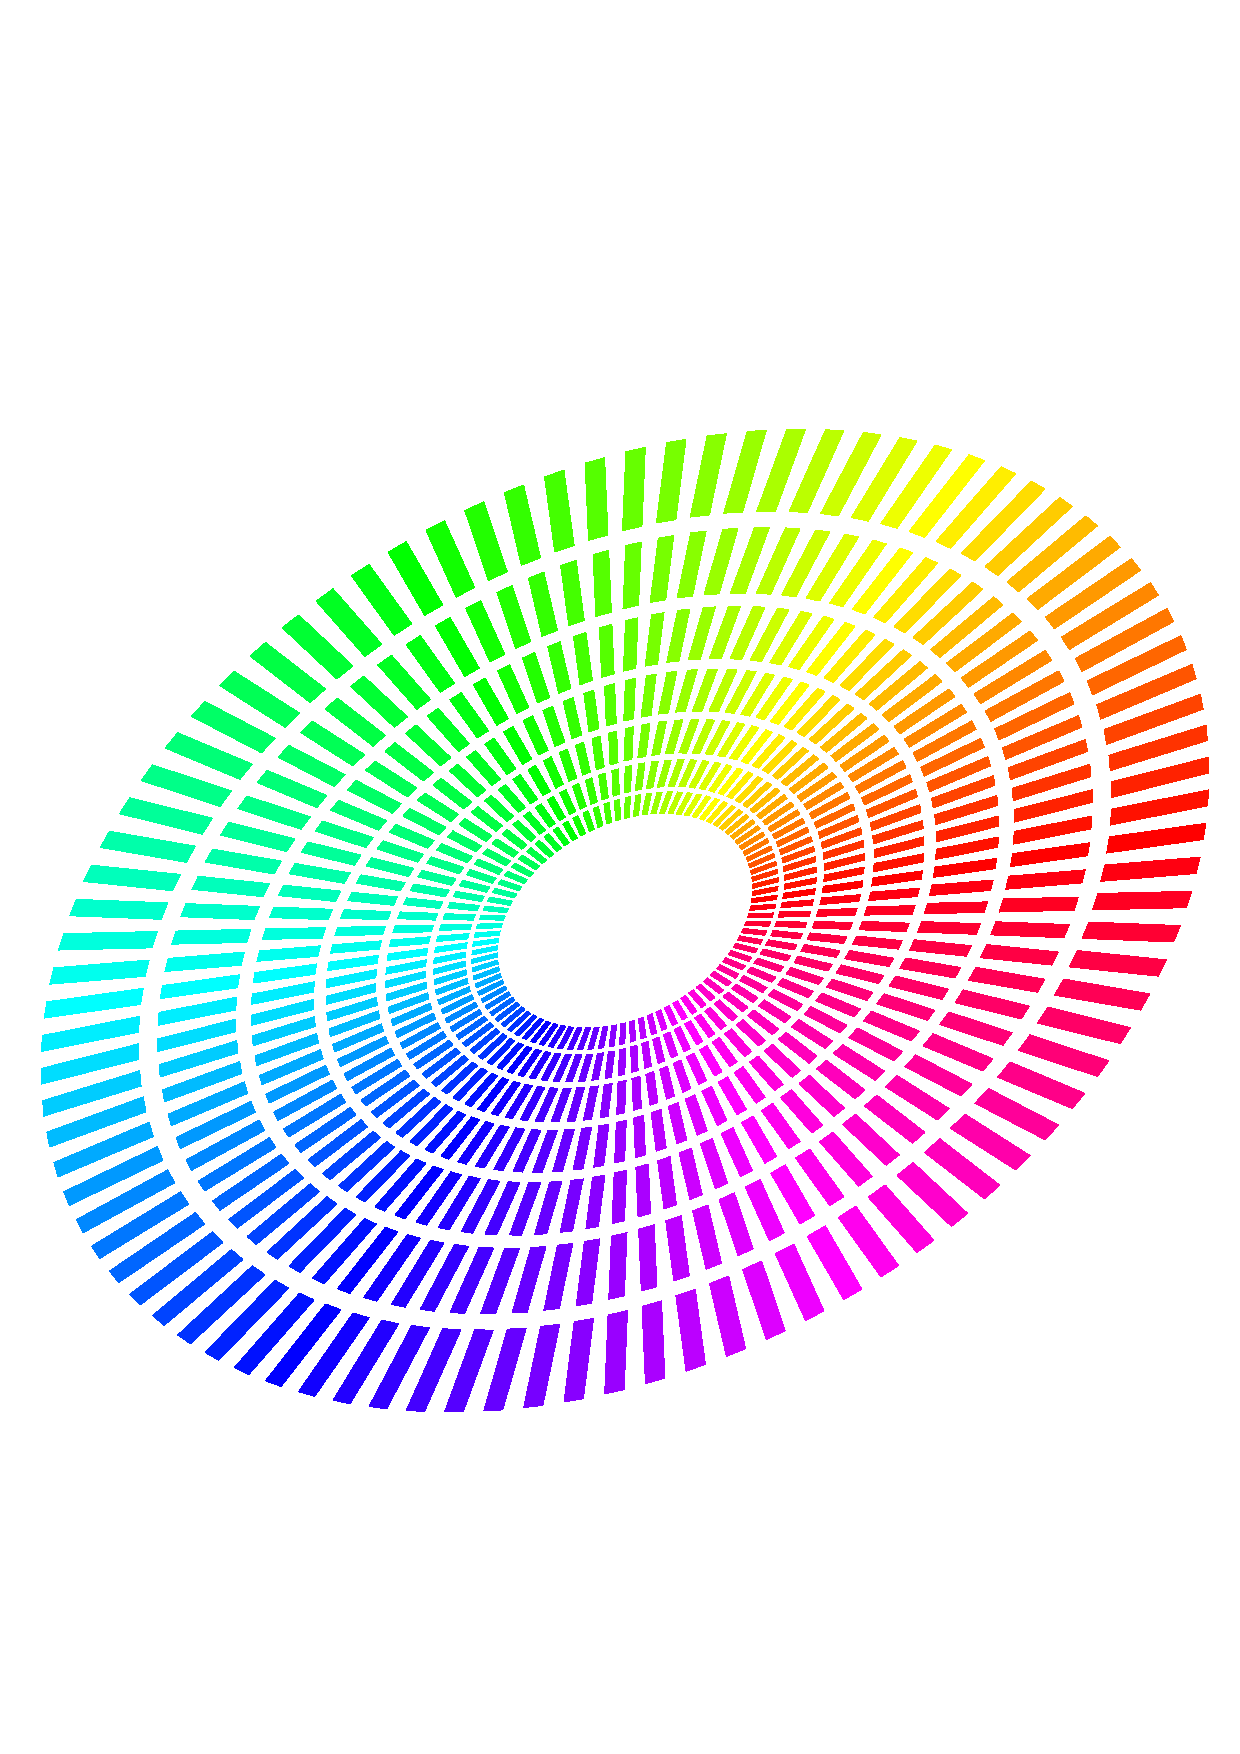
\includegraphics[width=4.2cm]{figure}
    \label{Figure:figsubex:right}
  }
  \caption{A doubly colourful picture.}
  \label{Figure:figsubex}
\end{figure}
%% ----------------------------------------------------------------
\section{Conclusions} \label{Section: Conclusions}
It works.
\acknowledgements{Thanks to no one.}
\backmatter
\bibliographystyle{ecs}
\bibliography{ECS}
\appendix
%% ----------------------------------------------------------------
\section{Stuff} \label{Section:Stuff}
The following gets in the way of the text....
\end{document}
%% ----------------------------------------------------------------
